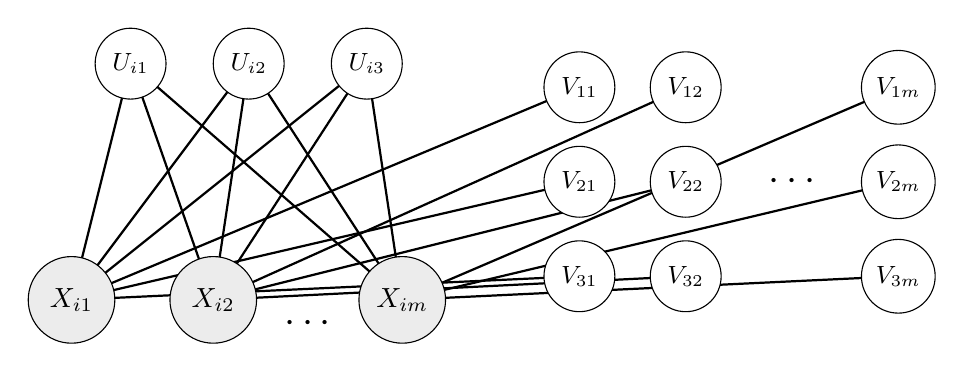
\begin{tikzpicture}[
    scale=1.5,
    node distance=1.5cm,
    observed/.style={circle, draw, fill=gray!15, minimum size=1.1cm, font=\normalsize},
    param/.style={circle, draw, fill=white, minimum size=0.9cm, font=\small}
]

% Arrows first (drawn behind)
% Arrows from U to all X
\draw[->, thick] (-1, 2) -- (-1.5, 0);
\draw[->, thick] (0, 2) -- (-1.5, 0);
\draw[->, thick] (1, 2) -- (-1.5, 0);

\draw[->, thick] (-1, 2) -- (-0.3, 0);
\draw[->, thick] (0, 2) -- (-0.3, 0);
\draw[->, thick] (1, 2) -- (-0.3, 0);

\draw[->, thick] (-1, 2) -- (1.3, 0);
\draw[->, thick] (0, 2) -- (1.3, 0);
\draw[->, thick] (1, 2) -- (1.3, 0);

% Arrows from V to X (gene 1)
\draw[->, thick] (2.8, 1.8) -- (-1.5, 0);
\draw[->, thick] (2.8, 1.0) -- (-1.5, 0);
\draw[->, thick] (2.8, 0.2) -- (-1.5, 0);

% Arrows from V to X (gene 2)
\draw[->, thick] (3.7, 1.8) -- (-0.3, 0);
\draw[->, thick] (3.7, 1.0) -- (-0.3, 0);
\draw[->, thick] (3.7, 0.2) -- (-0.3, 0);

% Arrows from V to X (gene m)
\draw[->, thick] (5.5, 1.8) -- (1.3, 0);
\draw[->, thick] (5.5, 1.0) -- (1.3, 0);
\draw[->, thick] (5.5, 0.2) -- (1.3, 0);

% Now draw nodes on top (U nodes as open circles)
\node[param] (u1) at (-1, 2) {$U_{i1}$};
\node[param] (u2) at (0, 2) {$U_{i2}$};
\node[param] (u3) at (1, 2) {$U_{i3}$};

% Multiple X nodes for different genes
\node[observed] (x1) at (-1.5, 0) {$X_{i1}$};
\node[observed] (x2) at (-0.3, 0) {$X_{i2}$};
\node[font=\Large] at (0.5, -0.2) {$\cdots$};
\node[observed] (xg) at (1.3, 0) {$X_{im}$};

% Parameters for gene 1 (reduced spacing)
\node[param] (v11) at (2.8, 1.8) {$V_{11}$};
\node[param] (v21) at (2.8, 1.0) {$V_{21}$};
\node[param] (v31) at (2.8, 0.2) {$V_{31}$};

% Parameters for gene 2
\node[param] (v12) at (3.7, 1.8) {$V_{12}$};
\node[param] (v22) at (3.7, 1.0) {$V_{22}$};
\node[param] (v32) at (3.7, 0.2) {$V_{32}$};

% Dots for more genes
\node[font=\Large] at (4.6, 1.0) {$\cdots$};

% Parameters for gene m
\node[param] (v1g) at (5.5, 1.8) {$V_{1m}$};
\node[param] (v2g) at (5.5, 1.0) {$V_{2m}$};
\node[param] (v3g) at (5.5, 0.2) {$V_{3m}$};

\end{tikzpicture}
